\documentclass{stdlocal}
\begin{document}
\section{Design and Implementation} % (fold)
\label{sec:design}

% Experimenting with various designs and implementations of algorithms, that robustly and efficiently smooth discrete curves on surface meshes, requires us to use a whole program pipeline or framework for loading input data, intuitively working with user interaction, and visualizing any intermediate results.
% As changing specific parts of such a pipeline may affect the performance, outcomes, and overall behavior of an algorithm or program, a brief overview over all of its components is essential to allow for reproducible results and will therefore be given in the following subsections.
% This will also make it possible for readers to simply reconstruct, adjust, and improve the pipeline for their own domain-specific projects.
% Afterwards, I will thoroughly elaborate on the design and implementation of chosen data structures and algorithms together with their mathematical primitives for curve smoothing.

% The pipeline or framework, described in this thesis, has been manually implemented with the C++ programming language and the OpenGL graphics API using some external libraries to handle low-level tasks.
% Already described in the introduction in section~\ref{sec:introduction}, this choice is well suited for open-source graphics applications and provides programmers with a large freedom when it comes to the implementation of data structures and algorithms.
% The complete source code of the project, called \textit{nanoreflex}, is provided as an open-source repository on GitHub.

The C++ code shown in this section does not provide the best design.

\subsection{Data Structures for Polyhedral Surfaces} % (fold)
\label{sub:polyhedral_surface_data_structure}

  In general, the choice and efficiency of algorithms highly depends on underlying data structures that represent the intermediate data of a program \autocite{knuth1997,mehlhorn2008,smed2006}.
  Thus, thorough design considerations for the data structures of polyhedral surfaces and surface mesh curves are mandatory to build fast and robust curve smoothing algorithms.
  Regarding the context of this thesis, I will focus on orientable polyhedral surfaces.
  As it was already explained before, this is not an actual restriction for the algorithm but will only speed up the implementation.
  Typical surfaces are the boundary of volumes that can be viewed as 3D open submanifolds of the 3D Euclidean space.
  These volumes must be oriented by construction and, hence, the boundary which represents the surface is oriented, too.

  To be able to render a triangular surface mesh in OpenGL, a simple and versatile method is to provide two separate lists for vertices and triangles, respectively \autocite{opengl}.
  Hereby, each triangle only references its three vertices by using indices that may be used to extract a vertex from the vertex list.
  The orientation of a triangle is defined by the order of its vertex references based on the description given in section~\ref{sec:preliminaries} in the preliminaries.
  Furthermore, vertices in OpenGL are quite general and may not only store their own positions.
  Typically, attributes for pseudo-normals, colors, or texture coordinates are added to use sophisticated shading techniques and improve the quality of illustrations.
  A concrete implementation of this can be seen in the following code snippet.
  Additionally, figure~\ref{fig:polyhedral-surface-faces} shows an example to visualize the memory layout of the vertex and face list.
  \inputCodeBlock[title = Vertices and Faces]{code/vertices-and-faces.hpp}

  \begin{figure}
    \centering
    \begin{subfigure}[c]{0.35\linewidth}
      \centering
      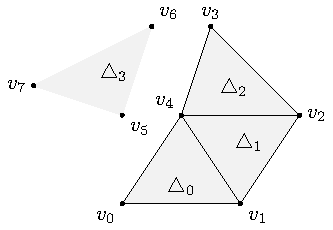
\includegraphics[width=\linewidth]{figures/polyhedral-surface-struct-base-scheme.pdf}
    \end{subfigure}
    \hfill
    \begin{subfigure}[c]{0.63\linewidth}
      \centering
      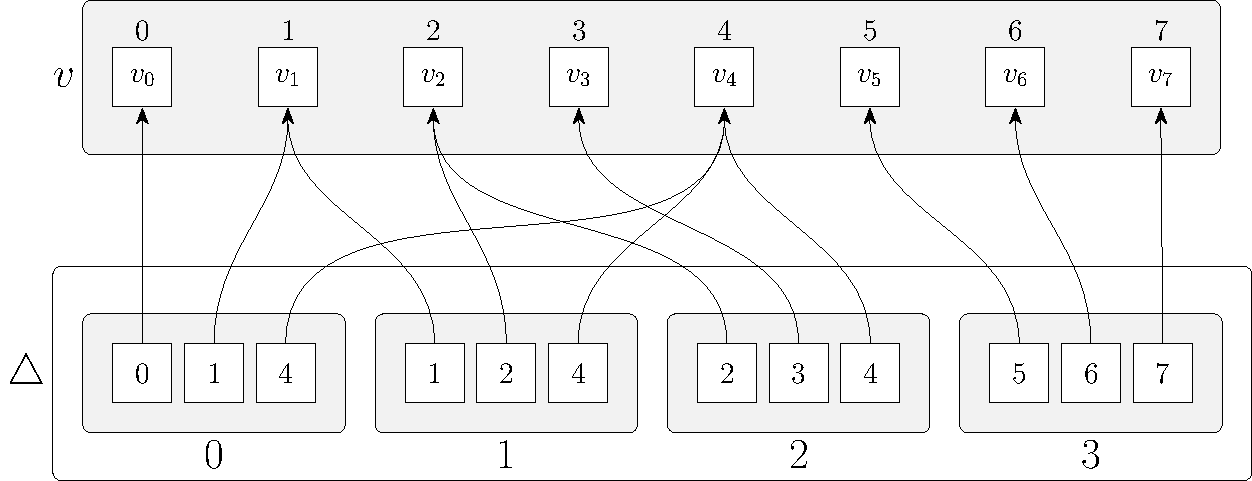
\includegraphics[width=\linewidth]{figures/polyhedral-surface-struct-base.pdf}
    \end{subfigure}
    \caption[Data Structure for Faces of a Polyhedral Surface]{%
      \textbf{Data Structure for Faces of a Polyhedral Surface}\\
      The figure shows a schematic example of how faces of a given polyhedral surface (left) are stored in memory.
      The surface consists of eight enumerated vertices and four faces.
      As it can be seen on the right, each face references three distinct vertices by their index in the order of their orientation.
      This way one vertex can be used by multiple triangles.
    }
    \label{fig:polyhedral-surface-faces}
  \end{figure}

  \noindent
  As polyhedral surfaces are a special form of 3D surface geometry, I will use file formats, such as STL \autocite{stl-file-format} and Wavefront OBJ \autocite{obj-file-format}, to provide the possibility for reading complex surface meshes from disk.
  Especially in the area of computer graphics in conjunction with the C++ programming language, the \textit{Assimp} library \autocite{assimp} is often used to load even more file formats that represent general surfaces and scenes.
  The facility makes it possible to test algorithms with very complex surface meshes from the \citetitle{thingi10k} dataset whose models are mainly provided as STL files.

  This representation already allows for an OpenGL-based visualization of polyhedral surfaces with sufficient quality by adding GLSL shaders.
  But in the context of this thesis, also the efficient movement of points and curves along the surface mesh needs to be possible.
  Over and over trying to determine adjacent neighbors of vertices or triangles with this data structure quickly becomes infeasible.
  So, further surface mesh preprocessing steps are needed to generate and store essential adjacency information.

  Computing and storing neighbor and adjacency information of surface meshes is a studied and vast area of computational geometry.
  There are multiple well-known data structures, like Quad-Edge Algebras \autocite{guibas1985} and triangular adjacencies \autocite{shewchuk1996}, for handling graphs that represent the topological structure of general 2D polyhedral surfaces.
  These data structures have successfully been used to efficiently construct Delaunay triangulations and encode the information of 3D surface meshes.
  The quad-edge algebra, described by \textcite{guibas1985}, is a versatile and complex data structure based on edges that represents both, the graph and the dual graph, of the surface at once and allows to easily and efficiently access the lists of adjacent vertices, edges, and faces.
  A simple but efficient implementation that does not make use of any pointers is given in section~\ref{sec:quad_edge_algebra} in the appendix.
  Figure~\ref{fig:quad-edge} and \ref{fig:quad-edge-rotation} schematically show the memory layout and rotation primitive of the data structure.
  On the other hand, according to \textcite{shewchuk1996}, a flat adjacency list storing references to adjacent faces for each face offers a lower memory consumption and an expected efficiency higher than that of a quad-edge algebra at the cost of a higher programming complexity when used in algorithms.
  It does not provide an easy way to access the graph but still incorporates the dual graph of the surface and is much easier to generate and handle than the quad-edge algebra.
  As each triangle may at most exhibit three other triangles that are adjacent to it, there is an upper storage bound for adjacency references of each triangle.
  Triangular adjacencies already have been used by \textcite{mancinelli2022} to implement one of the fastest geodesics tracing algorithms.
  Still, the adjacencies itself make it hard to access the circular list of adjacent faces around a vertex.
  My solution for triangular adjacencies, that will be explained in the following, uses insights gained from the quad-edge algebra and slightly changes the standard face references by adding locations to cope with this disadvantage.

  Unfortunately, the connectivity information provided by the faces and vertices are not suitable for surface mesh curves and smoothing algorithms.
  In an OpenGL-based rendering pipeline, the vertices of a polyhedral surface must differ as soon as they exhibit at least one distinct attribute.
  Even though triangles could share the same vertex position, their respective vertices might contain different pseudo-normals to model a crease in the surface and, consequently, these triangles cannot reference the same vertex.
  Even worse, for various reasons, it is allowed to use multiple instances of the same vertex inside the vertex list which also would lead to distinct vertex references.
  Especially, in the extreme case of STL files, every triangle uniquely refers to vertices that cannot be referred by other triangles which is schematically visualized in figure~\ref{fig:polyhedral-surface-distinct-vertices}.
  On the other hand, the values for additional attributes of a vertex, like pseudo-normals or texture coordinates, are unimportant for algorithms handling surface mesh curves and may be neglected as they do not change the topology of the underlying polyhedral surface.
  Such an algorithm would need to assume two vertices to be equivalent as long as they exhibit the same position.
  As a consequence, naively generating the graph or dual graph of the surface mesh solely based on the vertices and faces will not result in the correct topological connectivity needed for surface mesh curves.

  \begin{figure}[t]
    \centering
    \begin{subfigure}[c]{0.40\linewidth}
      \centering
      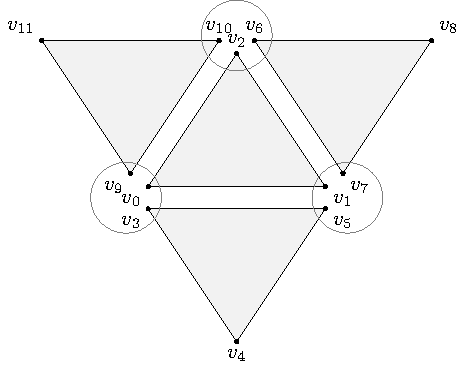
\includegraphics[width=\linewidth]{figures/polyhedral-surface-separated.pdf}
    \end{subfigure}
    \hfill
    $\longrightarrow$
    \hfill
    \begin{subfigure}[c]{0.40\linewidth}
      \centering
      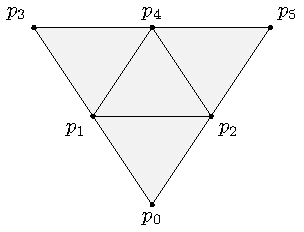
\includegraphics[width=\linewidth]{figures/polyhedral-surface-joint.pdf}
    \end{subfigure}
    \caption[Connectivity by Using Topological Vertices]{%
      \textbf{Connectivity by Using Topological Vertices}\\
      On the right, a simple polyhedral surface with six topological vertices and four faces is shown.
      In a data structure suitable for OpenGL-based rendering, each triangle might reference its own unique vertices as shown on the left.
      These vertices are distinct from each other which logically disconnects the four adjacent triangles.
    }
    \label{fig:polyhedral-surface-distinct-vertices}
  \end{figure}

  The use of surface mesh curves and smoothing algorithms should neither put a higher burden on the OpenGL pipeline nor require dramatic changes to data structures used for rendering.
  My solution to that problem generates an additional topological structure that extends the connectivity information given by the basic structure.
  Hereby, the main idea was that the projection of vertices onto their positions can be modeled by the quotient space and its respective quotient map.
  In this sense, let $\mathscr{V}$ be the set of all vertices and $\function{p}{\mathscr{V}}{\setReal^3}$ be the function that maps a vertex to its position in space.
  Two vertices $v,w\in\mathscr{V}$ are called to be topologically equivalent, denoted as $v\sim w$, if they exhibit the same position.
  \[
    v \sim w
    \quad :\iff\quad
    p(v) = p(w)
  \]
  Then the quotient space $\mathscr{V}/\sim$ consists of equivalence classes whose elements are pairwise topologically equivalent vertices.
  These equivalence classes will from now on be called topological vertices.
  The respective quotient map τ of $\mathscr{V}/\sim$ is given as follows.
  \[
    \function{τ}{\mathscr{V}}{\mathscr{V}/\sim}
    \separate
    τ(v) \define [v]
  \]
  Two triangles are topologically adjacent to each other if they share a topological edge and are not identical.
  Using the quotient map, a rigorous formulation can be given as follows.
  Let $n\in\setNatural$ be the number of vertices in the vertex list $\function{V}{\mathscr{I}}{\mathscr{V}}$ with $\mathscr{I}\define\set{k\in\setNatural_0}{k\leq n}$ as the index set.
  Two triangles of the faces list given by index triples $(v_1,v_2,v_3)$ and $(w_1,w_2,w_3)$ are adjacent to each other if there are permutations $σ,π\in\mathrm{S}_3$ such that the following holds.
  \[
    τ(V(v_{σ(1)})) = τ(V(w_{π(1)}))
    \separate
    τ(V(v_{σ(2)})) = τ(V(w_{π(2)}))
  \]
  \[
    τ(V(v_{σ(3)})) \neq τ(V(w_{π(3)}))
  \]
  Hence, by constructing the quotient map τ, I will be able to correctly determine topological connections.
  Still, the naive evaluation of the topological equivalence relation $\sim$ for all vertices is quadratic in complexity.
  For high-resolution polyhedral surfaces with millions of triangles, this is infeasible and needs to be addressed.

  My solution is based on a hash map in which all vertices will be inserted with respect to their position in space.
  As 3D vectors do not provide a natural order, a custom hash function needs to be used.
  Furthermore, the standard equality comparison is exchanged with the topological equivalence relation.
  This way topologically equivalent vertices are assumed to be the same by the hash map and are inserted at identical positions.
  Each insertion has an expected constant-time complexity.
  As a result, the insertion of all vertices exhibits a linear time complexity and offers a more efficient alternative to the naive method of checking pairwise equivalences.
  The following code snippet demonstrates a simple implementation of this method in C++.
  Additionally, figure~\ref{fig:polyhedral-surface-topological-vertex-map} schematically visualizes how the quotient map for the example given in figure~\ref{fig:polyhedral-surface-distinct-vertices} would look.

  \begin{figure}
    \centering
    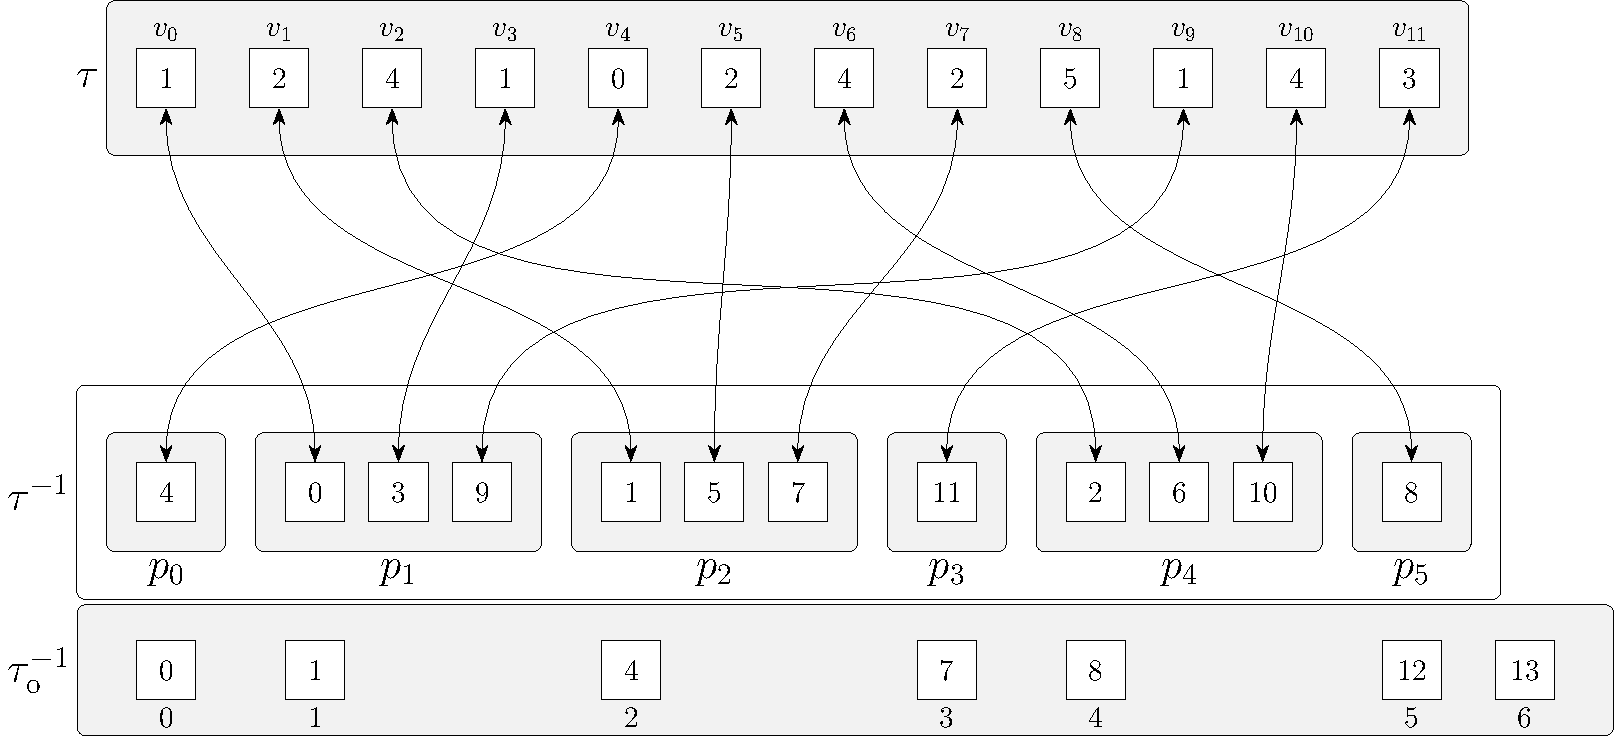
\includegraphics[width=\linewidth]{figures/polyhedral-surface-topological-vertex-map.pdf}
    \caption[Topological Quotient Map]{%
      \textbf{Topological Quotient Map}\\
      The figure schematically shows the quotient map τ of the polyhedral surface given in figure~\ref{fig:polyhedral-surface-distinct-vertices} which maps vertices onto their topological counterparts.
      As this map is not bijective, its inverse $τ^{-1}$ must use another array $τ^{-1}_\mathrm{o}$ of offsets.
    }
    \label{fig:polyhedral-surface-topological-vertex-map}
  \end{figure}

  \inputCodeBlock[title = Topological Vertex Map]{code/topological-vertex-map.hpp}

  \noindent
  With the above implementation, the inverse of the quotient map cannot directly be evaluated.
  This is a major drawback when working with edge-based data structures as these must reference topological vertices and there would be no efficient way to determine their position or shared pseudo-normals.
  If it is sufficient to access the positions of topological vertices then a simple copy of the positions might be the best way.
  In all other cases, the following code snippet provides a way to construct the inverse of the quotient map.
  Again, figure~\ref{fig:polyhedral-surface-topological-vertex-map} visualizes the inverse of the example given in figure~\ref{fig:polyhedral-surface-distinct-vertices}.
  As the quotient map is not bijective, an additional offset array is used to get the list of all vertices that refer to the same topological vertex.

  \inputCodeBlock[title = Inverse Topological Vertex Map]{code/inverse-topological-vertex-map.hpp}
  First, the code snippet calculates the cardinality of the equivalence classes representing topological vertices.
  Then by iteratively building the cumulative sum of cardinalities the data offset for each topological vertex has been determined.
  This offset is then used to add backwards pointing vertex references to the inverse map.
  As the offsets are changed by this operation, a final step shifts all the offsets to the left to repair the offset array.
  Getting all the vertex references of a topological vertex then only means to iterate over indices starting at the respective offset and ending before the next offset.

  With the availability of topological vertices and their correspondence to vertices, the next important intermediate construction step is the generation of all surface edges.
  During this construction step the given surface can be checked for orientability and consistency.
  Hereby, consistency means whether or not the vertices and faces fulfill the requirements of a 2D topological manifold.
  Furthermore, the intermediate representation of edges given below allows to determine nearly all the adjacency structures for vertices, edges, and faces.
  For this, a hash map of directed edges with a custom hash function for edges will be constructed by iterating over the list of faces.
  Hereby, each face will interpreted as an oriented triangle that adds all of its three directed edges to the hash map.
  The values for each directed edge in the hash map will refer to its specific triangle and its location inside that triangle.

  \inputCodeBlock[title = Intermediate Topological Edges]{code/topological-directed-edges.hpp}
  At the start of the code snippet structures for face adjacency references and directed edges are defined to simplify the implementation of edge generation.
  Directed edges are simply represented by two references to topological vertices.
  As they need to be added to a hash map, an information structure and a hash function have been added.
  The information structure only stores two face adjacencies to let the directed edge know from which face and at which location it originated.
  A face adjacency reference refers to a face in the face list and additionally to the edge location inside that face at which the adjacency occurs.
  As there are only three possible locations, only two bits are used to encode this information in the standard face reference by using the bit-field feature of C++.
  This reduces the amount of referencable faces to $2^{30}$ which is a little over 1~billion triangles.
  The memory consumption for this case would be $36\appendUnit{GiB}$ at minimum for the vertex and face list implementations provided here.
  Even nowadays graphics cards customary in trade are not able to handle this huge amount of data at once.
  Hence, the implementation does not impose serious constraints on the data it can handle.

  Now, to generate the topological face adjacencies, all that is to do is to iterate over all edges and add their mapped information to the face adjacencies.
  In the case that a triangle is part of the boundary of the polyhedral surface, a non-existing neighbor is marked as an invalid reference.
  The following code snippet demonstrates this.
  In figure~\ref{fig:polyhedral-surface-face-adjacencies}, a scheme that visualizes the memory layout of the topological face adjacencies can be seen.

  \begin{figure}
    \centering
    \begin{subfigure}[c]{0.38\linewidth}
      \centering
      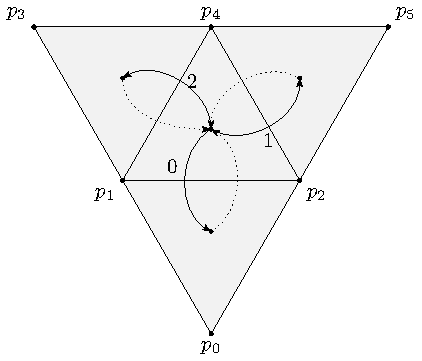
\includegraphics[width=\linewidth]{figures/polyhedral-surface-triangle-adjacencies.pdf}
    \end{subfigure}
    \hfill
    \begin{subfigure}[c]{0.60\linewidth}
      \centering
      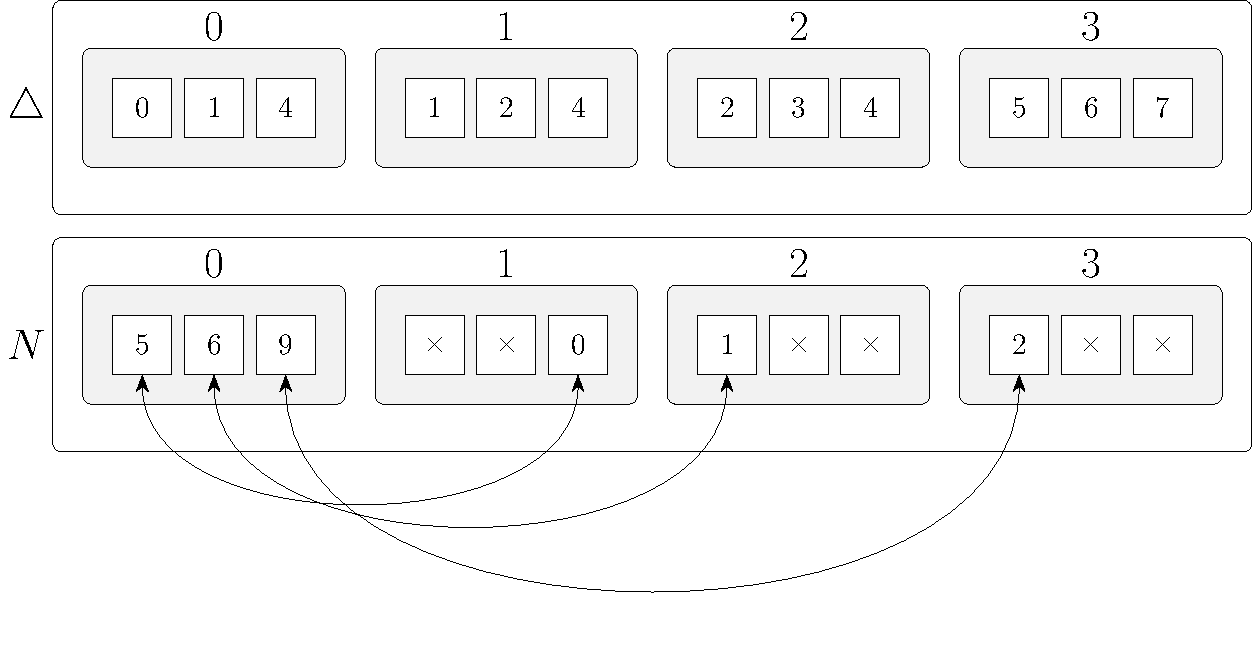
\includegraphics[width=\linewidth]{figures/polyhedral-surface-triangle-adjacencies-struct.pdf}
    \end{subfigure}
    \caption[Topological Face Adjacencies]{
      \textbf{Topological Face Adjacencies}\\
      The figure schematically visualizes how face adjacencies are stored in memory.
      On the left, the inner face of the polyhedral surface is surrounded by three other faces.
      For all these faces, its adjacency structure provides the face reference and the location inside their adjacency structure that points back to the inner face.
      In this example, the face adjacency is given by $N = 3f + l$ with $f$ as the face reference and $l$ as the location.
      Please note, in the code provided in this section, instead $N = 4f + l$ in the form of a bit-field is used for efficiency reasons.
    }
    \label{fig:polyhedral-surface-face-adjacencies}
  \end{figure}

  \inputCodeBlock[title = Topological Face Adjacencies]{code/topological-face-adjacencies.hpp}
  During the iteration over all directed edges, the code snippet distinguishes between oriented and unoriented edges.
  In the case of an oriented edge, the information structure only provides one valid face adjacency reference.
  Thus, the hash map of edges is queried for the reverse edge to get its information structure and with it the reference to the adjacent face.
  If the reverse edge does not exist, the current edge must be part of the boundary.

  Incorporating the location values into face adjacencies allows for an easy navigation along oriented polyhedral surfaces.
  Figure~\ref{fig:polyhedral-surface-face-adjacency-rotation} shows the basic operation for face adjacencies that rotates the current direction of the adjacency counterclockwise similar to quad-edge rotations of figure~\ref{fig:quad-edge-rotation}.
  It can be implemented by adding $1$ to the location and afterwards taking its modulus base $3$.
  This primitive enables the code to easily run through the list of triangles around a vertex in clockwise and counterclockwise order.
  Furthermore, for an algorithm which makes only use of the flat list of face adjacencies, the quotient map for topological vertices and the hash map for directed edges can be destroyed.
  In fact, the topological face adjacencies have been generated by the use of topological vertices but their data do not reference these anymore.

  \begin{figure}
    \centering
    \begin{subfigure}[c]{0.31\linewidth}
      \centering
      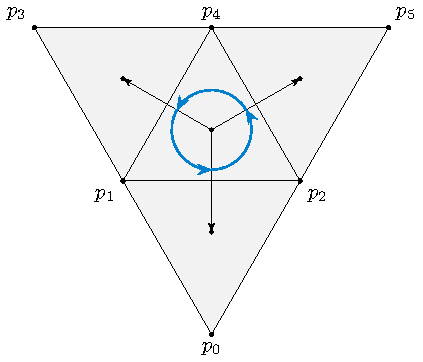
\includegraphics[width=\linewidth]{figures/polyhedral-surface-triangle-adjacencies-rot.pdf}
    \end{subfigure}
    \hfill
    \begin{subfigure}[c]{0.67\linewidth}
      \centering
      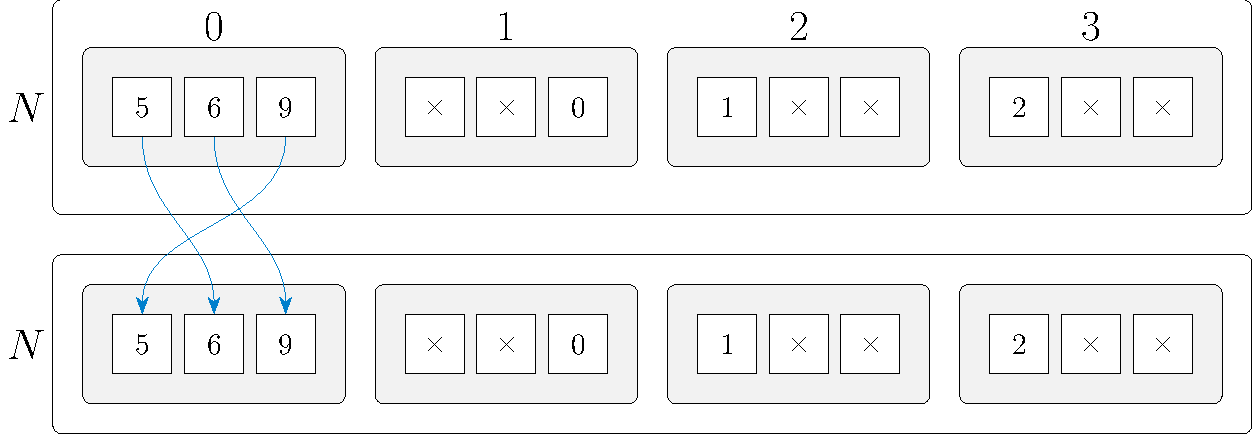
\includegraphics[width=\linewidth]{figures/polyhedral-surface-triangle-adjacencies-rot-struct.pdf}
    \end{subfigure}
    \caption[Counterclockwise Rotation of Topological Face Adjacencies]{
      \textbf{Counterclockwise Rotation of Topological Face Adjacencies}\\
      The rotation of face adjacencies (shown in blue) can be implemented by adding $1$ to the location and then taking its modulus base $3$.
      Using this operation together with all the face adjacencies allows to iterate through the list of faces around a vertex in clockwise and counterclockwise order.
    }
    \label{fig:polyhedral-surface-face-adjacency-rotation}
  \end{figure}

  As already described in section~\ref{sec:preliminaries} in the preliminaries, the vertices and edges of a polyhedral surface model a vertex-based graph which characterizes the vertex adjacencies.
  Looking at a polyhedral surface in this way, storing the triangle adjacencies makes the corresponding dual graph available.
  For the vertex-based graph, the adjacent vertices of each vertex would need be determined first.
  An efficient structure to store vertex neighbors is a sparse matrix in the compressed sparse row format without an extra array for matrix entries.
  The construction of counterclockwise oriented neighbor entries can be done by using the face adjacencies.
  Still, the boundary of a surface mesh needs to be handled by additional facilities as the vertex-based graph structure itself does not exhibit a way to simply encode them.
  Furthermore, the vertex-based graph needs to reference topological vertices and each vertex might have arbitrary many neighbors.

% subsection polyhedral_surface_data_structure (end)

\subsection{Data Structures for Surface Mesh Curves} % (fold)
\label{sub:discrete_surface_curve_data_structure}

  The representation of surface mesh curves via data structures may follow two main approaches and depends on the choice of data structures used to store topological adjacency information of the underlying polyhedral surface.

  \paragraph{Edge-Based Data Structure}\hfill\\
  On the one hand, surface mesh curves can solely be characterized by a list of control points over the surface mesh of a polyhedral surface.
  As the surface mesh is the union of topological edges, a natural construction would be based on a list of edges that contain the control points of the curve, respectively.
  To specify their exact position, an additional weighting parameter would need to be provided for every edge.
  Furthermore, in essence, the smoothing process can also be described as the movement of the curve along the surface.
  So, a feature is needed to map specific information of the initially given curve onto successive evolutions of the curve smoothing process.
  The following code snippet shows a simple implementation of these ideas.

  \inputCodeBlock[title = Edge-Based Surface Mesh Curve]{code/surface-mesh-curve-edge-based.hpp}
  Presumably, the code snippet above describes one of the easiest possible data structures as it represents a surface mesh curve directly as a list of control points.
  Hereby, the simple edge structure uses references to topological vertices and direction will always point to the right side of the curve on the surface.
  Closed curves can be represented by letting the last and the first point coincide.
  If the control point would need to represent a single vertex of the surface, both edge references should point to the same topological vertex.

  Unfortunately, this edge structure does not offer the ability to simply access adjacent edges or faces.
  Instead, all operations to change an edge and, as a consequence, the topology of the featured surface mesh curve are bound to either use the temporary hash map of directed edges or the adjacency structure for vertex neighbors in conjunction with a mask to identify boundary vertices.
  But using a sparse matrix of vertex neighbors, it is again possible to check for regularity of the surface mesh curve.
  In a regular surface mesh curve, three adjacent control points are not allowed to lie on the same triangle.
  For this, the edge of the next control point is not allowed to be the same as the edges of the current or previous control points.
  Additionally, it must also not be part of the edge that connects the edges of the previous and current control points.

  \paragraph{Face-Based Data Structure}\hfill\\
  On the other hand, triangle-based data structures have been successfully used before to implement surface mesh curves.
  The idea is basically to not directly reference edges but instead use their two adjacent triangles.
  Using this, not a list of edges with their weights is used but a strip of adjacent faces.
  Figure~\ref{fig:surface-mesh-curve-face-based} explains this principle by a schematic example.

  \begin{figure}
    \centering
    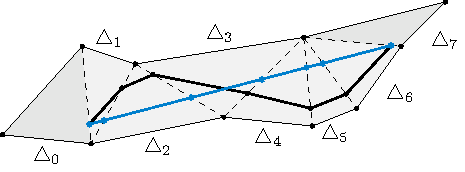
\includegraphics[width=0.8\linewidth]{figures/surface-mesh-curve.pdf}
    \caption[Face-Based Surface Mesh Curve]{%
      \textbf{Face-Based Surface Mesh Curve}\\
      The figure schematically shows an unfolded strip of adjacent triangles that are part of a polyhedral surface.
      Additionally, two surface mesh curves in black an blue are shown.
      Their control points are part of the edges of each pair of adjacent triangles.
      The blue surface mesh curve is also a discrete geodesic.
    }
    \label{fig:surface-mesh-curve-face-based}
  \end{figure}

  \inputCodeBlock[title = Face-Based Surface Mesh Curve]{code/surface-mesh-curve-face-based.hpp}
  Each face reference additionally stores the location of its previous adjacency and whether or not a right turn is next.
  As surface mesh curves do use essentially less points than polyhedral surfaces, it is not needed to encode the location information into the face reference itself.
  Using face references of the polyhedral surface, requires the implementation to separate the edge weights from the triangle strip.
  For a closed curve, only the last triangle needs to point to the first triangle and the first to the last.
  Additionally, another edge weight parameter would need to be added.
  The regularization of face-based surface mesh curves can be implemented in a much simpler way by making sure the next face is not the same as the previous or current face.
  For this structure, no topological vertices, edge hash maps or boundary maps are needed.
  A face-based representation is not generally applicable to surface mesh curves.
  They would need to at least provide some sort of regularity.
  But regular surface mesh are representable.

  \begin{figure}
    \centering
    \begin{subfigure}[c]{0.4\linewidth}
      \centering
      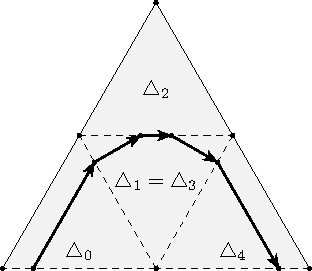
\includegraphics[width=\linewidth]{figures/surface-mesh-curve-artifact.pdf}
    \end{subfigure}
    \hfill
    $\longrightarrow$
    \hfill
    \begin{subfigure}[c]{0.4\linewidth}
      \centering
      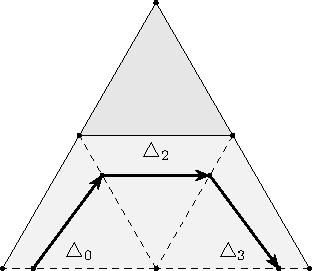
\includegraphics[width=\linewidth]{figures/surface-mesh-curve-artifact-removed.pdf}
    \end{subfigure}
    \caption[Regularization of Irregular Triangle Paths]{
      \textbf{Regularization of Irregular Triangle Paths}\\
    }
    \label{fig:surface-mesh-curves-face-based-regularization}
  \end{figure}

  \paragraph{Turn Compression}\hfill\\
  With the use of appropriate adjacency structures for a polyhedral surface, a surface mesh curve can be represented in a compressed structure that only contains the count of turns.
  Additionally, the first face adjacency needs to be stored as a starting point.
  Figure~\ref{fig:surface-mesh-curve-turns} schematically shows the idea behind the turn of a surface mesh curve.
  For the example given in figure~\ref{fig:surface-mesh-curve-face-based}, the turn scheme would be
  \[
    \textit{Right}
    \ \longrightarrow\
    \textit{Left}
    \ \longrightarrow\
    \textit{Right}
    \ \longrightarrow\
    \textit{Left}
    \ \longrightarrow\
    \textit{Left}
    \ \longrightarrow\
    \textit{Left}
  \]
  \[
    1\times\textit{Right}
    \ \longrightarrow\
    1\times\textit{Left}
    \ \longrightarrow\
    1\times\textit{Right}
    \ \longrightarrow\
    3\times\textit{Left}
  \]
  This representation is not as efficient to use for general smoothing but provides theoretical insights.

  \begin{figure}
    \centering
    \begin{subfigure}[b]{0.45\linewidth}
      \centering
      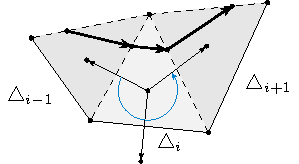
\includegraphics[width=\linewidth]{figures/surface-mesh-curve-rot-left.pdf}
      \caption{Left}
    \end{subfigure}
    \hfill
    \begin{subfigure}[b]{0.45\linewidth}
      \centering
      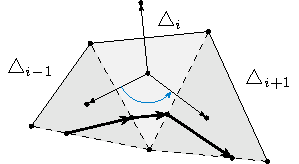
\includegraphics[width=\linewidth]{figures/surface-mesh-curve-rot-right.pdf}
      \caption{Right}
    \end{subfigure}
    \caption[Right and Left Turns of Surface Mesh Curves]{
      \textbf{Right and Left Turns of Surface Mesh Curves}\\
    }
    \label{fig:surface-mesh-curve-turns}
  \end{figure}

  % We do not look at polyhedral surfaces as an approximation of a real-world smooth manifold.

  % Advantages of discrete surface mesh curves over more general curves on polyhedral surfaces
  % \begin{itemize}
  %   \item Curve is provided in triangle precision. Better Compression. More points would be waste of memory.
  %   \item Robust: Snap to vertex if points get arbitrary near to each other
  %   \item curve is always a surface curve of the polyhedral surface and not violating mathematical properties. This also allows for direct rendering without projection.
  %   \item Useful for mesh processing
  %   \item Interpretation of Discretization is more consistent: surface mesh may be discretized approximationof real-world manifold with the mesh to be the finite grid. then it is only natural to discretize a real world surface curve in the same way.
  % \end{itemize}

  % Advantages of the triangular data structure over the edge-based one:
  % \begin{itemize}
  %   \item Triangles can be easier generalized to higher dimensions than edges.
  %   \item Triangles do not need to handle boundaries in complicated ways.
  %   \item Triangles allow easy and ordered access to fan around vertex.
  %   \item Artifact removal routine for triangles is simpler than for edges.
  %   \item Triangles do not exhibit data loss when handling reflex vertices
  %   \item Triangles allow for a more general moving of points
  % \end{itemize}

  \begin{figure}
    \centering
    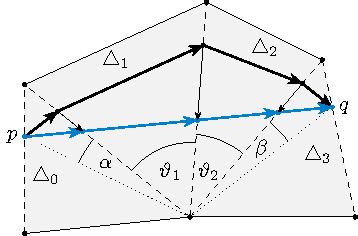
\includegraphics[width=0.5\linewidth]{figures/unfolding-critical-vertex.pdf}
    \caption[Unfolding Critical Vertex]{%
      \textbf{Unfolding Critical Vertex}\\
    }
  \end{figure}

% subsection discrete_surface_curve_data_structure (end)

\subsection{Smoothing of Surface Mesh Curves} % (fold)
\label{sub:smoothing_of_surface_mesh_curves}
  The overall procedure consists of two main primitives.
  Reflections at reflex vertices and local smoothing.
% subsection smoothing_of_surface_mesh_curves (end)

% \subsection{Overview of the Program Pipeline} % (fold)
% \label{sub:program_pipeline}
%   In the following, the stages of the implemented program pipeline are stated and summarized.
%   These stages naturally arise from an insight into the generation and tracing of geodesics on surface meshes, described in section~\ref{sec:previous_work}.
%   Locally shortest or straightest geodesics that follow as a solution from the discrete boundary value problem are in some sense the smoothest curves that cannot be made any smoother.
%   As we typically need to provide an initial curve for those geodesics to be found, the whole generation and tracing of geodesics can be looked at as an extreme smoothing process.
%   Adding parameters to let the user decide on when to stop this process then results in the pipeline given below and schematically shown in figure~\ref{fig:program-pipeline}.

%   \begin{figure}[h]
%     \begin{center}
%       \large
%       INSERT YOUR IMAGE HERE!
%     \end{center}
%     \caption[Program Pipeline Stages]{%
%       \textbf{Program Pipeline Stages}\\
%       The scheme shows all the stages of the implemented program pipeline.
%       The arrows indicate data flow and dependencies.
%     }
%     \label{fig:program-pipeline}
%   \end{figure}

%   \begin{enumerate}
%     \item \textbf{Surface Mesh Loading:}\\
%       Load a surface mesh given by a specific file format from the storage.
%     \item \textbf{Surface Mesh Preprocessing:}
%       \begin{enumerate}
%         \item Generate a connected mesh object to properly model the topology of the input.
%         \item Generate the pseudo-normals for each vertex.
%         \item Generate the dual graph for the neighbors of each triangle.
%         \item Check that the mesh is a valid orientable two-dimensional topological manifold.
%       \end{enumerate}
%     \item \textbf{Initial Curve Selection:} \\
%       Let the user choose an initial curve by drawing on the surface.
%     \item \textbf{Parameter Selection:} \\
%       Let the user choose parameters for the curve smoothing algorithm.
%     \item \textbf{Curve Smoothing:} \\
%       Smooth the initial curve according to the constraints given by the selected parameters.
%     \item \textbf{Postprocessing:} \\
%       Optionally apply the smoothed curve in a domain-specific context.
%   \end{enumerate}
%   According to figure~\ref{fig:program-pipeline}, the output of every stage is not only forwarded to the next stage but also specifically visualized and rendered to the screen to provide the user with visual feedback and to catch errors or exceptional behavior as early as possible.
%   Besides, additional user interactions will be processed for all stages to allow for measurements and adjustments and to be able to react to the output of previous stages.
%   The loading of surface meshes from different file formats is typically handled by loader libraries, such as \textit{Assimp}, and will not be further explained.
%   On the other hand, surface mesh preprocessing and the initial curve selection are crucial steps in the whole pipeline which remove geometric degeneracies and artifacts that would otherwise violate assertions needed for the correct execution of the algorithm.
%   Therefore both stages will be discussed in more detail in the following subsections.
%   The postprocessing in our case is optional and only provided for the sake of completeness.
%   The parameter selection is highly dependent on the implementation of the curve smoothing algorithm and, as a result, it will be described together with the curve smoothing itself.
% % subsection program_pipeline (end)

% \subsection{Surface Mesh Preprocessing} % (fold)
% \label{sub:mesh_preprocessing}
%   The goal of preprocessing a surface mesh which has been loaded from disk is to transform its data into a valid and efficient representation of a polyhedral surface that should exhibit functionality to draw and move points and discrete curves on its surface.
%   In the case that this transformation is not possible, the stage at least must check for the validity of the given data and emit an error if there might be any violations.
%   % On one hand, the preprocessing of a given surface mesh needs to make sure that the program or algorithm is actually dealing with a valid two-dimensional topological manifold.

%   A given Mesh for the algorithm can be quite general.
%   Providing triangles which will introduce numerical difficulties is out of the scope of this thesis.

%   We will focus on orientable meshes.
%   Please note, that is not an actual restriction for the algorithm but will only speed up the implementation.
%   Furthermore, we look at surfaces which are the boundary of volumes in three-dimensional Euclidean space which can be looked at as open submanifolds.
%   These volumes are therefore by definition oriented and, hence, their boundary needs to be, too.
%   Still, we need to look boundaries for surfaces as, for example, distance envelopes restrict the surface without boundary to be one.
%   The boundaries need to be handled properly.
%   Also, these requirements are only need to hold for the restriction to the distance envelope.
%   Often, lines will be drawn on oriented/orientable parts of the surface even if the surface is not orientable due to artifacts originating from scanning or generating meshes.

%   \paragraph{Topological Connections}
%   We need the topological connections of a given surface mesh.
%   In the case of general file formats, a scene is typically separated into multiple meshes which are topologically but not smoothly connected.
%   For proper drawing of curves in a whole scene, the topological structure of connections needs to be generated first.
%   Using the STL file format, this is not needed.

%   \paragraph{Generating the dual graph}
%    To generate such a dual graph we refer to this book.
%   It is assumed to be a solved problem.
%   First, we have created a hash map of oriented edges with a custom hash function to mangle vertex indices.
%   The mapped values store the faces indices and their location in the triangle.
%   By inverting the indices of a stored edge, one can easily access the neighboring triangle if it exists.
%   Furthermore, it is easy to check whether the mesh is oriented and a valid two-dimensional manifold.

%   \paragraph{Check for orientability and validity}

% % subsection mesh_preprocessing (end)

\subsection{Initial Curve Selection} % (fold)
\label{sub:initial_curve_selection}
  As for the vast majority of optimization algorithms, the results and efficient working are highly dependent on the chosen starting values.
  Curve smoothing itself is an optimization process and to solve the boundary value problem, we need an initial value.
  So, choosing the initial curve in the right way will also heavily change the speed and quality of the algorithm.
  The algorithm should be able to handle a vast amount unsmooth curves.
  Still, the handling of artifacts will be taken care of at the start.
  \paragraph{User Interface for Selecting and Controlling Initial Curves}
  \paragraph{Drawing by Ray Tracing}
  \paragraph{Connecting the Vertices}
  \paragraph{Closed Initial Curves and Fixed Vertices}
  \paragraph{Artifact Removal}
  \paragraph{Smoothed Curvature Values by Stencil}
    Stencil is discrete approximation of solution to Laplacian equation or heat equation which is smooth (infinitely differentiable).
    Maybe it would be useful to keep the length of the curve and still smooth it.
  \paragraph{Vertex Curves}
  \paragraph{Face Curves}
  \paragraph{Tracing Geodesics}
% subsection initial_curve_selection (end)

\subsection{Unfolding} % (fold)
\label{sub:unfolding}
To unfold two triangles along their common edge and find the shortest line connecting two points, we will first look back into two dimensions.

\begin{figure}[h]
  \centering
  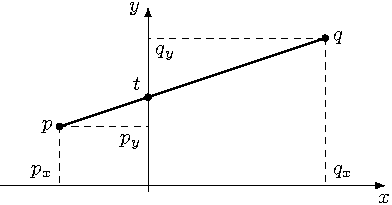
\includegraphics[width=0.6\linewidth]{figures/unfolding_geodesic_2d.pdf}
  \caption[2D Unfolding Primitive]{%
    \textbf{2D Unfolding Primitive}
  }
\end{figure}

Let $p,q\in\setReal^2$ such that $p_x < q_x$.
\[
  \Delta x = q_x - p_x
  \separate
  \Delta y = q_y - p_y
  \separate
  \Sigma x = p_x + q_x
  \separate
  \Sigma y = p_y + q_y
\]
The straight line function connecting these two points then looks like the following.
\[
  f(x) = \frac{q_y - p_y}{q_x - p_x}(x - p_x) + p_y = \frac{q_y - p_y}{q_x - p_x}x + \frac{p_yq_x - q_yp_x}{q_x - p_x}
\]
Please note that this function is well-defined, as $q_x - p_x > 0$.
To get the intersection point with the ordinate, set the argument to zero.
\[
  t\define f(0) = \frac{p_yq_x - q_yp_x}{q_x - p_x} = \frac{\Delta x \Sigma y - \Sigma x \Delta y}{2 \Delta x}
\]
\begin{figure}[h]
  \begin{subfigure}[b]{0.49\linewidth}
    \centering
    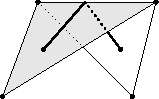
\includegraphics[width=0.9\linewidth]{figures/unfolding_geodesic.pdf}
    \caption{Folded in 3D space}
  \end{subfigure}
  \hfill
  \begin{subfigure}[b]{0.49\linewidth}
    \centering
    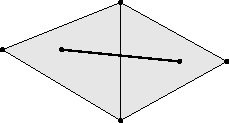
\includegraphics[width=\linewidth]{figures/unfolding_unfolded.pdf}
    \caption{Unfolded in 2D space}
  \end{subfigure}
  \caption[Unfolding of two Triangles]{%
    \textbf{Unfolding of two Triangles}
  }
  \label{fig:design-triangle-unfolding}
\end{figure}

Applying this expression to the case of two triangles that needs to be unfolded, the following results.
\[
  e \define \frac{v_2 - v_1}{\norm{v_2 - v_1}}
  \separate
  p \define r_1 - v_1
  \separate
  q \define r_2 - v_1
\]
\[
  p_y = \scalarProduct{e}{p}
  \separate
  q_y = \scalarProduct{e}{q}
\]
\[
  p_x = -\norm{p - p_y e}
  \separate
  q_x = \norm{q - q_y e}
\]
Unfolding two adjacent triangles that share a common edge from three-dimensional space into the two-dimensional plane is not unique as there are two cases.
In one case, the triangles might overlap and in the other not.
The above sign for $p_x$ is therefore important.

\begin{lemma}[Unfolding leads to geodesic]
  Connecting $p$, $r$, and $q$ in that order by straight lines leads to locally shortest and straightest geodesics as long as $λ\in (0,1)$.
  It solves the discrete boundary value problem for locally shortest and straightest geodesics when boundary points lie in the inside of adjacent triangles.
\end{lemma}
\begin{proof}
  According to \textcite{polthier2006} and \textcite{martinez2005}, locally shortest and straightest geodesics coincide on polyhedral if they do not contain any vertices.
  So, it is sufficient to show that the discrete curvature at the crease is zero.
  But this has be true by construction.
\end{proof}
% subsection unfolding (end)

\subsection{Unfolding with Desired Curvature} % (fold)
\label{sub:unfolding_with_desired_curvature}

  \begin{figure}[h]
    \centering
    \begin{subfigure}[b]{0.49\linewidth}
      \centering
      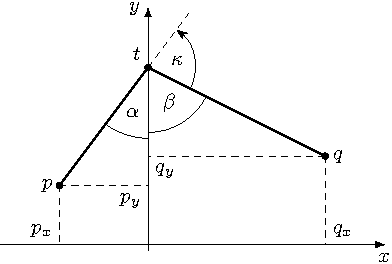
\includegraphics[width=\linewidth]{figures/unfolding_curvature_2d.pdf}
      \caption{$κ < 0$}
    \end{subfigure}
    \hfill
    \begin{subfigure}[b]{0.49\linewidth}
      \centering
      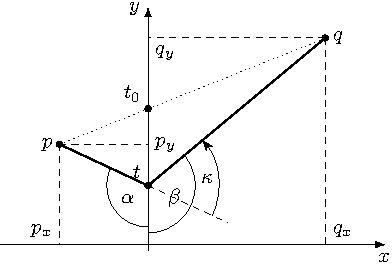
\includegraphics[width=\linewidth]{figures/unfolding_curvature_2d_positive.pdf}
      \caption{$κ > 0$}
    \end{subfigure}
    \caption[2D Unfolding Curvature Primitive]{%
      \textbf{2D Unfolding Curvature Primitive}\\
    }
    \label{fig:}
  \end{figure}

Again, a two-dimensional primitive is used.
\[
  f(x) = -\cot α (x - p_x) + p_y
\]
\[
  t = f(0) = p_y + \absolute{p_x}\cot α
\]
Now, combine two points to both sides with a desired discrete curvature.
For this, assume $p_x < 0$ and $q_x > 0$.
Furthermore, the desired curvature is positive $κ > 0$ and taken mathematically positive.
$α,β\in(0,π)$ and $κ\in(-π,π)$ with $κ < α$ and $π+κ > α$
\[
  κ + π = α + β
\]
From the former computation, it is clear that their points on the ordinate have to coincide.
\[
  p_y - p_x \cot α = q_y + q_x \cot β
\]
\[
  \cot β = \cot(π-(α-κ)) = -\cot(α-κ)
\]
\[
  \cot(α-κ) = \frac{\cos κ \cot α + \sin κ}{\cos κ - \sin κ \cot α}
\]
% \[
%   \cot(α-κ) = \frac{\cot α \cot κ + 1}{\cot κ - \cot α}
% \]
% \[
%   p_y - p_x \cot α = q_y - q_x \frac{\cot α \cot κ + 1}{\cot κ - \cot α}
% \]
\[
  φ\define \cot{α}
  % \separate
  % K\define \cot κ
\]
\[
  p_y - p_x φ = q_y - q_x \frac{φ \cos κ + \sin κ}{\cos κ - φ \sin κ}
\]
\[
  q_x \frac{φ \cos κ + \sin κ}{\cos κ - φ \sin κ} = q_y - p_y + p_x φ
\]
\[
  φ q_x \cos κ + q_x \sin κ
  = (\Delta y + φ p_x)(\cos κ - φ \sin κ)
\]
\[
  φ q_x \cos κ + q_x \sin κ
  = \Delta y \cos κ - φ \Delta y \sin κ + φ p_x \cos κ - φ^2 p_x \sin κ
\]
\[
  φ^2 p_x \sin κ + φ (\Delta x \cos κ + \Delta y \sin κ) + q_x \sin κ - \Delta y \cos κ = 0
\]
\[
  φ = \frac{1}{2 p_x \sin κ} \boxBrackets{-(\Delta x \cos κ + \Delta y \sin κ) \pm \sqrt{(\Delta x \cos κ + \Delta y \sin κ)^2 - 4p_x \sin κ (q_x \sin κ - \Delta y \cos κ)}}
\]
\[
  φ = \frac{1}{2 p_x \sin κ} \boxBrackets{-(\Delta x \cos κ + \Delta y \sin κ) \pm \sqrt{(\Sigma x \cos κ + \Delta y \sin κ)^2 - 4 p_x q_x}}
\]
\[
  t = \frac{1}{2 \sin κ} \boxBrackets{\Delta x \cos κ + \Sigma y \sin κ \pm \sqrt{(\Sigma x \cos κ + \Delta y \sin κ)^2 - 4 p_x q_x}}
\]
\[
  t = t_0 + \Delta t
\]
\[
  t = t_0 + \frac{1}{2 \sin κ} \boxBrackets{-2t_0\sin κ + \Delta x \cos κ + \Sigma y \sin κ \pm \sqrt{(\Sigma x \cos κ + \Delta y \sin κ)^2 - 4 p_x q_x}}
\]
\[
  t_0 = \frac{1}{2}(\Sigma y - \Sigma x \frac{\Delta y}{\Delta x})
\]
\[
  \Delta t = \frac{1}{2 \sin κ} \boxBrackets{\Sigma x \frac{\Delta y}{\Delta x}\sin κ + \Delta x \cos κ \pm \sqrt{(\Sigma x \cos κ + \Delta y \sin κ)^2 - 4 p_x q_x}}
\]
\[
  2 \Delta t \sin κ \leq 0
\]
\[
  \Delta t = \frac{1}{2 \sin κ} \boxBrackets{\Sigma x \frac{\Delta y}{\Delta x}\sin κ + \Delta x \cos κ - \sqrt{(\Sigma x \cos κ + \Delta y \sin κ)^2 - 4 p_x q_x}}
\]
% \[
%   Kq_xφ + q_x = \Delta y φ - K\Delta y + p_x φ^2 - Kp_x φ
% \]
% \[
%   q_x + K\Delta y = p_x φ^2 + (\Delta y -K(p_x+q_x))φ
% \]
% \[
%   \frac{q_x + K\Delta y}{p_x} = φ^2 + \frac{\Delta y - K\Sigma x}{p_x}φ
% \]
% \[
%   φ = -\frac{\Delta y - K\Sigma x}{2p_x} \pm \sqrt{\frac{q_x + K\Delta y}{p_x} + \frac{(\Delta y - K\Sigma x)^2}{4p^2_x}}
% \]
% \[
%   t = p_y - p_x φ
% \]
% \[
%   t = p_y + \frac{\Delta y - K\Sigma x}{2} \mp \sqrt{p_x(q_x + K\Delta y) + \frac{(\Delta y - K\Sigma x)^2}{4}}
% \]
% \[
%   t = \frac{\Sigma y - K\Sigma x}{2} \mp \sqrt{p_x(q_x + K\Delta y) + \frac{\Delta^2y - 2K\Delta y\Sigma x + K^2\Sigma^2x}{4}}
% \]
% \[
%   t = \frac{\Sigma y - K\Sigma x}{2} \mp \sqrt{p_xq_x(1 + K^2) + \frac{\Delta^2y - 2K\Delta y\Delta x + K^2\Delta^2x}{4}}
% \]
% \[
%   t = \frac{\Sigma y - K\Sigma x}{2} \mp \sqrt{p_xq_x(1 + K^2) + \frac{(\Delta y - K\Delta x)^2}{4}}
% \]
% subsection unfolding_with_desired_curvature (end)

\subsection{Desired Curvature Stencil} % (fold)
\label{sub:desired_curvature_stencil}

% subsection desired_curvature_stencil (end)

\subsection{Desired Curvature Mapping} % (fold)
\label{sub:desired_curvature_mapping}

% subsection desired_curvature_mapping (end)

\subsection{Curve Smoothing Algorithm} % (fold)
\label{sub:curve_smoothing_algorithm}
  Curve smoothing is not a discrete problem.
  Using only a finite amount of steps is probably not possible.
  So, we use a process of convergence.
  This has the advantage that not all triangles need to be unfolded at once.
  This makes the implementation and parallelization much simpler.
  The discrete algorithms for tracing geodesics are not easy to parallelize.

  \paragraph{Idea and Overview}
  \paragraph{Edge Vertex Relaxation}
    We need to take a look at topological and numerical robustness.
  \paragraph{Vertex Vertex Relaxation}
  \paragraph{Critical Vertex Handling}
  \paragraph{Artifact Removal and Self-Intersection Handling}
  \paragraph{Desired Curvature Mapping}
    Desired curvatures need to be constant along edges.
    Therefore interpolate on angle-basis around vertex.
    We do not want to loose information of desired curvatures.
  \paragraph{Curve Evaluation}
  \paragraph{Correctness and Convergence}
    Correctness can be shown by showing the convergence to the curvature values.
    This by definition of the given curvature values smooths the curve.
    The convergence might only be shown for contracting the curve by smoothing.
    As the limit is the geodesic, the prove of its convergence is there.
  \paragraph{Complexity}
% subsection curve_smoothing_algorithm (end)

% section design (end)
\end{document}
